% LMM Proposal Hackathon Chip 2026 -- LaTeX port of proposal.html
% Build: pdflatex proposal.tex (figures in figs/)
\documentclass[9pt]{extarticle}
\usepackage[a4paper,margin=11mm,left=12mm,right=12mm]{geometry}
\usepackage[T1]{fontenc}
\usepackage[utf8]{inputenc}
\usepackage[indonesian]{babel}
\usepackage{helvet}
\renewcommand{\familydefault}{\sfdefault}
\usepackage{amsmath,amssymb}
\usepackage{graphicx}
\usepackage[table]{xcolor}
\usepackage{tabularx,array,booktabs}
\usepackage{enumitem}
\usepackage{titlesec}
\usepackage{caption}
\usepackage{multicol}
\usepackage[framemethod=default]{mdframed}
\usepackage[hidelinks]{hyperref}

\definecolor{acc}{HTML}{1F4E8C}
\definecolor{mut}{HTML}{56606B}
\definecolor{line}{HTML}{C9D1DA}
\definecolor{bg2}{HTML}{F2F5F9}
\definecolor{thbg}{HTML}{E4EBF3}
\definecolor{ok}{HTML}{1D6B3C}
\definecolor{bad}{HTML}{A3271F}

\setlength{\parindent}{0pt}
\setlength{\parskip}{0.8mm}
\linespread{1.08}
\setlist{nosep,leftmargin=5mm}
\captionsetup{font={scriptsize,color=mut},labelfont={scriptsize,color=mut},justification=raggedright,singlelinecheck=false,skip=1mm}
\renewcommand{\figurename}{Gambar}

\titleformat{\section}{\color{acc}\bfseries\large}{}{0pt}{}[{\color{acc}\titlerule[0.6pt]}]
\titlespacing*{\section}{0pt}{3.2mm}{1.2mm}
\titleformat{\subsection}{\bfseries\normalsize}{}{0pt}{}
\titlespacing*{\subsection}{0pt}{2.2mm}{0.8mm}

\arrayrulecolor{line}
\renewcommand{\arraystretch}{1.15}
\setlength{\tabcolsep}{1.1mm}
\newcolumntype{L}{>{\raggedright\arraybackslash}X}
\newcolumntype{R}{>{\raggedleft\arraybackslash}X}
\newcommand{\hd}[1]{\cellcolor{thbg}\textbf{#1}}
\newcommand{\ok}[1]{\textcolor{ok}{\textbf{#1}}}
\newcommand{\bad}[1]{\textcolor{bad}{\textbf{#1}}}
\newcommand{\code}[1]{\colorbox{bg2}{\footnotesize\texttt{#1}}}
\newcommand{\note}[1]{{\color{mut}\scriptsize #1}}

\newmdenv[backgroundcolor=bg2,linecolor=acc,topline=false,bottomline=false,rightline=false,
  linewidth=2pt,innerleftmargin=2mm,innerrightmargin=2mm,innertopmargin=1mm,innerbottommargin=1mm,
  skipabove=1.2mm,skipbelow=1.2mm]{callout}

\begin{document}
\footnotesize

{\color{acc}\Large\bfseries PROPOSAL PESERTA HACKATHON CHIP 2026}\\[0.5mm]
{\color{mut}\small Kategori: IC Chip Design \& FPGA Implementation $\cdot$ Topik 03 AI/Edge Accelerator (dengan Security Design sebagai fondasi)}

\vspace{1.5mm}
{\scriptsize
\begin{tabularx}{\linewidth}{|p{0.22\linewidth}|L|}
\hline
\hd{Judul Ide Desain Chip} & \textbf{LMM-16: Secure, Low-Power Tiled INT16 Matrix Engine untuk Inferensi Typed-Decision Laya pada DE10-Nano} \\ \hline
\hd{Nama Tim} & [diisi tim] \\ \hline
\hd{Anggota Tim (2--4)} & Ketua: [Nama] -- [Institusi] -- [Email/HP] $\cdot$ Anggota 1: [\dots] $\cdot$ Anggota 2: [\dots] \\ \hline
\hd{Dosen Pembimbing} & [Nama Dosen \& Gelar] -- [Institusi] \\ \hline
\end{tabularx}}

\note{Label angka: \textbf{[U]} hasil ukur/simulasi di repo ini $\cdot$ \textbf{[S]} spesifikasi resmi $\cdot$ \textbf{[E]} estimasi $\cdot$ \textbf{[A]} asumsi. Semua skrip dan hasil mentah: \texttt{fpga/} (RTL, testbench, \texttt{fpga/results/*.json}).}

% ---------------------------------------------------------------
\section{1. Ringkasan Ide (Executive Summary)}
\textbf{Masalah yang diangkat.} Laya multilingual (321.908.995 parameter [U]) adalah model \emph{typed-decision}: teks bebas + pilihan dinamis $\rightarrow$ probabilitas keputusan, tanpa API eksternal. Profiling CPU kami menunjukkan satu bentuk kernel, \code{Y[L,2304] = X[L,768]$\cdot$W[768,2304]} (44 pemanggilan per inferensi: 22 \code{attn.Wqkv} + 22 \code{mlp.Wi}, bobot berbeda per layer), memakan \textbf{35--41\% waktu operator} [U]. Pada CPU edge kecil (Cortex-A9 800\,MHz [S]) beban ini menjadi penghambat utama inferensi lokal.

\textbf{Solusi yang ditawarkan.} IP \textbf{LMM-16}: mesin GEMM ter-\emph{tile} yang mengambil tile X/W dari DDR HPS, menghitung 128 MAC/siklus dengan DSP Cyclone V, dan menulis akumulator INT32 kembali ke DDR. Host tetap menjalankan tokenizer, operator lain, dan keputusan. Bobot tetap berupa \emph{data} di DDR, bukan logika.

\textbf{Implementasi pada DE10-Nano.} Kontrol melalui \emph{lightweight} HPS-to-FPGA (CSR 32-bit). Data melalui dua port FPGA-to-SDRAM 64-bit (baca X/W, tulis Y), dengan \emph{completion} lewat IRQ f2h. Satu domain clock 100\,MHz; CDC ditangani bridge hard HPS [S].

\textbf{Kebaruan \& keunggulan yang dapat dibuktikan} (bukan klaim kecepatan sebelum uji board):
\begin{enumerate}
\item \textbf{Presisi berbasis bukti.} Gate keputusan Laya menunjukkan INT8 membalik 2 dari 12 keputusan. Kontrak \textbf{W16A16} mempertahankan 12/12 keputusan pada biaya DSP \textbf{sama} dengan INT8, karena multiplier native Cyclone V adalah 18$\times$18.
\item \textbf{Keamanan di RTL}: jendela DMA terkunci, validasi \emph{fail-closed} sebelum transaksi bus pertama, \emph{guard} lapis-2 di tiap burst, dan \emph{scrub} seluruh buffer. 32/32 test negatif lolos [U].
\item \textbf{RTL bit-exact} terhadap reference integer pada 72 tensor Laya nyata dan pada inferensi penuh dengan RTL di dalam loop [U].
\item Utilisasi compute 97,6--97,9\% dan perilaku \code{max(compute, transfer)} dibuktikan lewat simulasi sweep bandwidth [U].
\end{enumerate}

% ---------------------------------------------------------------
\section{2. Latar Belakang \& Rumusan Masalah}
\textbf{Latar belakang.} Brief proyek mengarahkan pada akselerator untuk kernel dominan, bukan memindahkan 322M parameter ke RTL. Bukti profiling (CPU M1, FP32, 4 thread, 12 pesan $\times$ panjang state 64/128/256/512; panjang gabungan L = 109/173/301/557 untuk skema uji):

{\scriptsize
\begin{tabularx}{\linewidth}{|R|R|R|R|R|R|}
\hline
\hd{L} & \hd{Kernel 768$\rightarrow$2304, ms/inferensi [U]} & \hd{\% aten self-CPU [U]} & \hd{aten::mm total [U]} & \hd{Median e2e, 360 run acak [U]} & \hd{MAC/pemanggilan} \\ \hline
109 & 29,4 & 41,3\% & 59,6\% & 66 ms & 192.872.448 \\ \hline
173 & 35,5 & 40,5\% & 58,5\% & 88 ms & 306.118.656 \\ \hline
301 & 55,1 & 38,7\% & 55,7\% & 136 ms & 532.611.072 \\ \hline
557 & 95,0 & 35,2\% & 50,6\% & 256 ms & 985.595.904 \\ \hline
\end{tabularx}}

\textbf{Rumusan masalah \& batasan.}
\begin{enumerate}
\item \textbf{Bobot tidak muat on-chip.} Satu matriks INT16 berukuran 3,54\,MB, sedangkan total M10K hanya 553 blok ($\approx$553\,KB) [S]. Bobot harus di-stream dari DDR3 32-bit yang dipakai bersama CPU (puncak teoretis 400\,MHz $\times$ 2 $\times$ 32 bit = 3,2\,GB/s [S, diturunkan]).
\item \textbf{Presisi.} Kandidat harus mereproduksi keputusan \emph{baseline}, termasuk 4 keputusan baseline yang salah; label tidak diperbaiki.
\item \textbf{Keamanan.} Master F2S dapat mengakses seluruh SDRAM [S]. Bug atau proses jahat bisa mengubah akselerator menjadi DMA liar.
\item \textbf{Amdahl.} Dengan porsi 35--41\%, percepatan end-to-end pada platform yang sama dibatasi $\le$ 1,54--1,69$\times$ [D].
\end{enumerate}

\textbf{Gap.} Karya DE10-Nano terdekat (Gadea-Giron\'es dkk., 2024 [1]) memakai kernel OpenCL FP32 untuk CNN, mencapai 95--108\,MHz pada utilisasi logic 90\%. Penulisnya menyimpulkan HPS+NEON ``hardly justif[ies] the use of the FPGA'' kecuali FPGA membebaskan CPU, dan jalur DDR antar-kernel mendominasi. Belum ada GEMM transformer yang presisinya dipilih dari gate keputusan, aman terhadap DMA, dan bit-exact.

\begin{callout}
\textbf{Gate numerik: mengapa implementasi memakai INT16, bukan INT8} (dijalankan sebelum RTL; baris selain W16A16 adalah alternatif yang \underline{ditolak}, bukan implementasi). 44 modul Laya diganti kernel kandidat; 12 kasus; dibandingkan dengan baseline FP32 pada proses yang sama [U, \texttt{fpga/results/e2e\_*.json}].

{\scriptsize
\begin{tabularx}{\linewidth}{|p{0.26\linewidth}|R|R|R|L|}
\hline
\hd{Kandidat} & \hd{Error relatif tensor (median)} & \hd{Keputusan sama} & \hd{max$|\Delta p|$} & \hd{Catatan} \\ \hline
W8A8 per-kanal/per-token & 3,4e-2 & \bad{10/12} & 0,223 & billing\_512, other\_512 terbalik \\ \hline
W8 + aktivasi FP32 & 7,8e-3 & \bad{10/12} & 0,057 & error bobot INT8 sudah cukup membalik \\ \hline
BF16 (operand), akumulasi FP32 & 1,8e-3 & \bad{11/12} & 0,0074 & margin baseline 0,012 sangat tipis \\ \hline
W12A12 / W14A14 & 2,1e-3 / 5,2e-4 & \ok{12/12} & 0,0053 / 0,0014 & lolos tipis / aman \\ \hline
\textbf{W16A16 + $\gg$10 $\rightarrow$ INT32 (kontrak)} & 1,3e-4 & \ok{12/12} & 0,0005 & setara FP16 (1,6e-4); \textbf{dipilih} \\ \hline
\end{tabularx}}

Literatur konsisten: aktivasi BERT memiliki outlier sehingga W8A8 PTQ gagal tanpa penanganan khusus [7]; LLM.int8() memindahkan outlier ke matmul 16-bit [8].
\end{callout}

% ---------------------------------------------------------------
\section{3. Proposed Chip Design}
\subsection{3.1 Solusi \& Arsitektur Sistem}

\begin{figure}[h!]
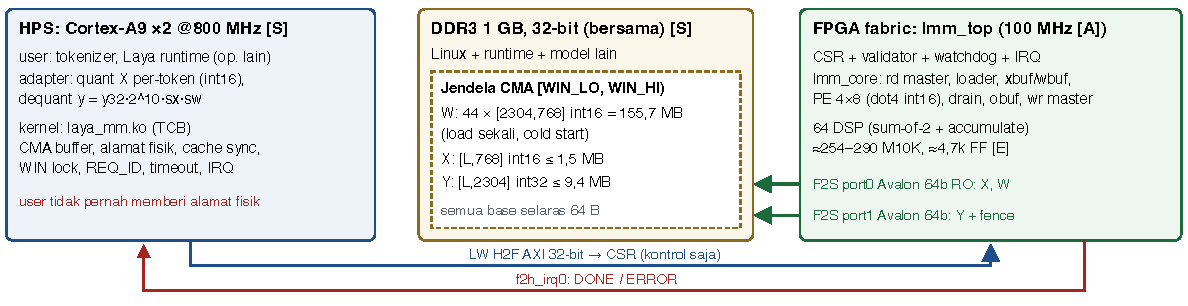
\includegraphics[width=\linewidth]{figs/fig1.pdf}
\caption{Partisi sistem. Jalur kontrol (LW, 32-bit) terpisah dari jalur tensor (F2S, 2$\times$64-bit). Tidak dipakai: H2F AXI 128 (CPU menjadi penyalin data) dan F2H/ACP (koheren tetapi melewati L2 dan bersaing dengan cache CPU; F2S terukur jauh lebih cepat [2]).}
\end{figure}

\begin{figure}[h!]
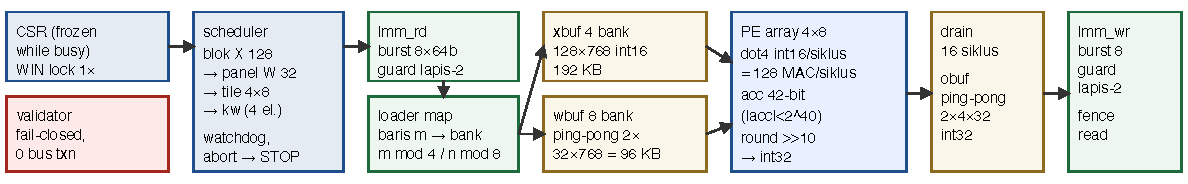
\includegraphics[width=\linewidth]{figs/fig2.pdf}
\caption{Arsitektur internal IP. Setelah DONE, ERROR, atau abort, \texttt{lmm\_scrub} menulis nol ke xbuf, wbuf, obuf, akumulator, dan register drain (6.144 siklus = 61\,\textmu s).}
\end{figure}

\subsection{Kontrak numerik, pemrosesan, dan alasan pemilihan}
$q_x = \mathrm{clip}(\mathrm{rint}(x/s_x), \pm 32767)$ dengan $s_x$ per token; $q_w$ per kanal keluaran, dikuantisasi offline. $\mathit{acc} = \sum_k q_x \cdot q_w$ eksak dengan $|\mathit{acc}| < K\cdot 2^{30} \le 2^{40}$, sehingga akumulator 42-bit tidak bisa overflow (validator menjaga $K \le 768$). Keluaran $y_{32} = (\mathit{acc} + 2^{9}) \ggg 10$ (round-half-up, $|y_{32}| < 2^{30}$) muat di INT32 tanpa saturasi. Host melakukan dequant: $y = y_{32}\cdot 2^{10}\cdot s_x\cdot s_w$.

\textbf{Mengapa 16-bit?} DSP Cyclone V mengalikan 18$\times$18 secara native (2 per blok, mode sum + akumulator 64-bit [S, 3, 4]). Jadi INT16 tidak menambah DSP dibanding INT8; biayanya hanya traffic W 2$\times$ dan BRAM 2$\times$. Ini lebih murah daripada kehilangan keputusan.

\textbf{Lima level yang dipisahkan:}
\begin{enumerate}
\item Golden FP32 PyTorch.
\item Reference integer \code{lmm\_ref.py}.
\item RTL. Wajib bit-exact terhadap level 2.
\item Adapter simulator \code{rtl\_kernel.py}. Kontraknya \code{matmul(x,w)} FP32$\rightarrow$FP32, sama dengan \code{verification\_v1.py}.
\item Driver HPS di board (rencana).
\end{enumerate}

\subsection{Arsitektur memori \& penempatan blok (dengan perhitungan)}
{\scriptsize
\begin{tabularx}{\linewidth}{|p{0.17\linewidth}|p{0.25\linewidth}|>{\raggedleft\arraybackslash}p{0.11\linewidth}|L|}
\hline
\hd{Data} & \hd{Lokasi} & \hd{Ukuran} & \hd{Justifikasi} \\ \hline
Bobot Wqkv/Wi 44 matriks & DDR, CMA milik driver; RO bagi FPGA & 155,7 MB & tidak muat on-chip; tidak di-mmap ke user (integritas) \\ \hline
X blok ($T_M$=128 baris) & xbuf M10K, 4 bank (baris m $\rightarrow$ bank m mod 4) & 192 KB & dipakai ulang oleh 72 panel W (N/32); W dibaca $\lceil L/128\rceil$ kali \\ \hline
W panel ($T_N$=32 baris) $\times$2 & wbuf M10K, 8 bank, ping-pong & 96 KB & panel p dihitung saat p+1 dimuat; $T_N$ minimum yang masih overlap \\ \hline
Segmen Y & obuf M10K, ping-pong & 2 KB & compute tidak menunggu tulis \\ \hline
Akumulator, drain & register (DSP acc + FF) & 32$\times$42\,b + 32$\times$32\,b & di-scrub tiap request \\ \hline
Deskriptor & register CSR (bukan di DDR) & 15$\times$32\,b & dibekukan saat busy: tanpa TOCTOU \\ \hline
\end{tabularx}}

\textbf{Pemilihan tile.} Traffic W per pemanggilan adalah $\lceil L/T_M\rceil\times$3,54\,MB. Untuk L=557 [D]:

{\scriptsize
\begin{tabularx}{\linewidth}{|r|r|r|L|}
\hline
\hd{$T_M$} & \hd{xbuf} & \hd{Traffic W} & \hd{Kesimpulan} \\ \hline
64 & 96 M10K & 31,9 MB & traffic W terbesar \\ \hline
\textbf{128} & 192 M10K & 17,7 MB & \textbf{dipilih}: $T_M$ terbesar yang masih menyisakan margin \\ \hline
256 & 384 M10K & 10,6 MB & tidak muat bersama wbuf ($>$ 553) \\ \hline
\end{tabularx}}

$T_N$ tidak mengubah traffic. Ia hanya menentukan ukuran wbuf dan syarat overlap: compute per panel 24.576 siklus harus $\ge$ muat panel 6.144 beat + tulis 2.048 beat. $T_N$=32 memenuhi syarat dengan wbuf terkecil (96 M10K), sehingga daya statis/dinamis BRAM lebih rendah.

\textbf{Packing M10K.} Kebutuhan bit ideal: xbuf 1,57\,Mbit = 154 blok, wbuf 0,79\,Mbit = 77 blok. Mode 256$\times$40 atau 512$\times$20 untuk word 64-bit menjadi 192 + 96 + 2 = 290 blok (batas atas). Yosys memetakan 254 blok (46\%) [E].

\subsection{Komunikasi, register map, dan urutan satu request}
{\scriptsize
\begin{tabularx}{\linewidth}{|p{0.13\linewidth}|p{0.27\linewidth}|L|}
\hline
\hd{Interface} & \hd{Spesifikasi resmi [S]} & \hd{Pilihan \& alasan} \\ \hline
LW HPS-to-FPGA & AXI 32-bit tetap, base 0xFF20\_0000 (2 MB) & CSR Avalon 32-bit; latensi rendah, terisolasi dari data \\ \hline
FPGA-to-SDRAM (F2S) & AXI-3/Avalon-MM, $\le$ 6 port, 32/64/128/256 bit per port; MPFE bersama & 2 port Avalon 64-bit. Kebutuhan rata-rata 297--359 MB/s [U] = 37--45\% puncak port 64-bit @100 MHz. 128/256-bit hanya menambah ALM, routing, dan daya tanpa throughput (compute-bound). Pengukuran Cyclone V: F2S jauh lebih cepat dari F2H, dan seluruh transfer FPGA$\rightarrow$HPS $<$ 1.500 MB/s [2]; R+W serentak 20,08 Gbps [5]. \\ \hline
Reset/CDC & bridge HPS punya clock crossing asinkron; port F2S dilepas lewat \texttt{fpgaportrst} (0xFFC2\_5080) saat SDRAM idle & satu clock 100 MHz; reset async-assert/sync-release; urutan: konfigurasi FPGA $\rightarrow$ bridge $\rightarrow$ \texttt{fpgaportrst} (U-Boot) $\rightarrow$ probe driver \\ \hline
\end{tabularx}}

{\scriptsize
\textbf{Register map} (word offset): 0x00 ID $\cdot$ 0x01 CTRL (START, ABORT, IRQ\_EN, CLR) $\cdot$ 0x02 STATUS \{err\_code, rejected, err, done, busy, state\} $\cdot$ 0x03/0x04 REQ\_ID/DONE\_ID $\cdot$ 0x05--0x07 M, K, N $\cdot$ 0x08--0x0A alamat X, W, Y $\cdot$ 0x0B TIMEOUT $\cdot$ 0x0C--0x0E WIN\_LO, WIN\_HI, WIN\_LOCK $\cdot$ 0x10--0x13 PERF (siklus, siklus MAC, beat baca, beat tulis).

\textbf{Urutan request dan kepemilikan buffer:}
\begin{enumerate}
\item \textbf{Host.} Kuantisasi X ke slot CMA, lalu \code{ioctl(SUBMIT)}. Driver menulis CSR, REQ\_ID, START. X, W, dan Y berpindah milik ke device.
\item \textbf{CHECK.} Bila gagal, kirim ERROR dengan 0 beat bus.
\item \textbf{LDX.} Muat blok X.
\item \textbf{LDW.} Muat panel 0.
\item \textbf{PANEL.} Compute panel p sambil memuat panel p+1. Segmen Y ditulis segera setelah drain.
\item \textbf{FLUSH, lalu fence read.} Satu baca alamat Y terakhir di port yang sama, supaya DONE tidak mendahului data.
\item \textbf{SCRUB.} Lalu DONE, DONE\_ID=REQ\_ID, dan IRQ.
\item \textbf{Driver.} Cocokkan DONE\_ID (completion basi ditolak), lalu \code{dma\_sync\_for\_cpu(Y)}. Buffer kembali milik user.
\end{enumerate}}

\subsection{Security Design (fondasi, bukan tempelan)}
{\scriptsize
\textbf{Threat model.}
\begin{itemize}
\item \textbf{Dipercaya:} bitstream, kernel, dan driver.
\item \textbf{Tidak dipercaya:} proses user/adapter, dimensi, dan isi tensor.
\item \textbf{Aset:} memori DDR proses lain/kernel (paling kritis), teks pelanggan dalam X/Y (privasi), integritas bobot dan hasil.
\item \textbf{Batas:} bila root/kernel kompromi, isolasi hilang (bisa reprogram FPGA atau memakai \code{/dev/mem}). Proteksi port di SDRAM controller dicatat sebagai lapis-3 opsional.
\item \textbf{Tanpa kriptografi:} bobot Laya publik, dan checksum bukan autentikasi.
\end{itemize}

\begin{tabularx}{\linewidth}{|p{0.22\linewidth}|p{0.22\linewidth}|L|}
\hline
\hd{Ancaman} & \hd{Ditegakkan driver} & \hd{Ditegakkan RTL (diuji)} \\ \hline
DMA di luar buffer & user hanya memberi slot & WIN terkunci; validator; guard per burst di rd/wr (kode 4, 9) \\ \hline
Overflow alamat/ukuran & hitung 64-bit & ujung region 34-bit; Y=0xFFFF\_FFC0 ditolak \\ \hline
Dimensi ilegal & cek & $1\le M\le 1024$; $64\le K\le 768$, $K\,\%\,32=0$; $32\le N\le 2304$, $N\,\%\,32=0$; TIMEOUT$>0$ \\ \hline
Overlap berbahaya & slot terpisah & $Y\cap X = \emptyset$ dan $Y\cap W = \emptyset$ (kode 5) \\ \hline
Deskriptor berubah / request saat busy & mutex & argumen beku saat busy; START/tulis ditolak dan diberi flag \\ \hline
Hang, abort di tengah burst & timeout $\rightarrow$ ABORT $\rightarrow$ reset bridge & watchdog (7), ABORT (8): berhenti issue, terima sisa beat, burst tidak terpotong \\ \hline
Completion basi / residu data & cek DONE\_ID & DONE\_ID hanya saat sukses; scrub semua buffer; fault dibersihkan saat scrub \\ \hline
\end{tabularx}}

\subsection{Daya rendah sebelum optimasi}
{\scriptsize
\begin{itemize}
\item \textbf{Reuse} menekan traffic DDR. X dipakai 72$\times$; W dipakai 32 tile baris per blok.
\item \textbf{Clock enable dan operand isolation.} RAM hanya membaca saat \code{issue}; register dot/acc hanya aktif saat valid. Tidak ada gated clock di fabric.
\item \textbf{Port 64-bit}, bukan 128/256.
\item \textbf{128 lane, bukan 224.} 224 lane butuh $\approx$525 MB/s rata-rata, sedangkan sweep menunjukkan lebar pita bersama menjadi batas.
\item \textbf{IRQ, bukan busy-poll.}
\end{itemize}

\textbf{Metrik dibedakan:} idle, dinamis (Quartus Power Analyzer + aktivitas simulasi), daya total board, dan energi per inferensi. Belum ada angka watt hasil ukur.

\textbf{Referensi daya [1]:} board DE10-Nano 3,72\,W saat ARM-only dan 7,45\,W dengan desain FPGA aktif. Jadi energi hanya menang bila latensi turun $>\approx$2$\times$.}

\subsection{Rincian modul RTL (Verilog-2001, total 585 baris)}
{\scriptsize
\begin{tabularx}{\linewidth}{|p{0.13\linewidth}|r|L|}
\hline
\hd{Modul} & \hd{Baris} & \hd{Fungsi \& invarian} \\ \hline
lmm\_top & 162 & CSR Avalon, validator \emph{fail-closed}, WIN lock, watchdog, PERF, IRQ, reset sync \\ \hline
lmm\_core & 274 & FSM IDLE$\rightarrow$LDX$\rightarrow$LDW$\rightarrow$PANEL$\rightarrow$FLUSH$\rightarrow$FENCE$\rightarrow$SCRUB (STOP saat abort); loader map; PE 4$\times$8 dot4; drain; ping-pong \\ \hline
lmm\_rd / lmm\_wr & 52 / 80 & master burst Avalon; guard lapis-2; outstanding dibatasi 256 beat (counter tidak wrap); fence \\ \hline
lmm\_ram & 17 & RAM dual-port, baca terdaftar dengan enable (inferensi M10K) \\ \hline
\end{tabularx}

Custom ISA tidak diperlukan: operasinya satu (GEMM) dengan layout tetap, sehingga register cukup dan permukaan serangan lebih kecil.}

\subsection{Estimasi penggunaan resource FPGA}
{\scriptsize
\begin{tabularx}{\linewidth}{|p{0.17\linewidth}|R|R|r|}
\hline
\hd{Komponen} & \hd{Estimasi (Yosys \texttt{synth\_intel\_alm} Cyclone V) [E]} & \hd{Kapasitas 5CSEBA6 [S]} & \hd{\%} \\ \hline
Logic (ALM) & 13,8k LUT $\approx$ 7--9k ALM & 41.910 ALM (110K LE) & 17--22 \\ \hline
Register & 4.674 FF & 166.036 & 2,8 \\ \hline
Block RAM (M10K) & 254 (batas atas 290) & 553 blok / 5.570 Kb & 46--52 \\ \hline
DSP & 128 mult. 18$\times$18 array = 64 blok; +3 validator & 112 blok / 224 mult. & 57--60 \\ \hline
Clock target & 100 MHz [A] & DSP mode sum 250 MHz ($-$I7) [3] & -- \\ \hline
\end{tabularx}

Catatan: template menulis register 415.000; Device Overview resmi menyebut 166.036 [S]. Angka Yosys bukan hasil fit Quartus. Fmax baru sah setelah timing closure. Karya HLS sebanding menutup timing pada 95--108\,MHz walau logic-nya 90\% terpakai [1].

\textbf{Tools:} Icarus Verilog 13 + GTKWave (unit/keamanan/waveform), Verilator 5.052 (replay besar, $\approx$200$\times$ Icarus), Python/NumPy/PyTorch (reference, gate), Yosys 0.69 (estimasi), Intel Quartus Prime Lite + Platform Designer + SignalTap (board; butuh host Linux/Windows x86).}

\subsection{3.2 Rencana Pengujian \& Hasil Simulasi (MacBook Air M1)}
{\scriptsize
\begin{tabularx}{\linewidth}{|p{0.15\linewidth}|L|p{0.33\linewidth}|}
\hline
\hd{Uji} & \hd{Isi} & \hd{Hasil [U]} \\ \hline
Keamanan (\texttt{+test=sec}) & start tanpa lock, 8 argumen ilegal, misalign, luar window, wrap 4 GB, overlap X/W, tulis saat busy, DONE\_ID, IRQ, watchdog, abort, guard lapis-2 (bound dirusak setelah validasi), pemulihan, scrub $\times$3 & \ok{32/32 lolos di Icarus \& Verilator; request ditolak = 0 beat bus; monitor 0 pelanggaran} \\ \hline
Bentuk \& stall acak & $M\in\{1,3,4,5,9,31,127,128,129,130\}$, K 64--256, N 32--96, magnitudo terburuk $\pm$32767, stall 0/20/60\%, latensi 1/8/30 & \ok{10/10 bit-exact} \\ \hline
Fixture Laya & 72 tensor nyata (12 kasus $\times$ layer 0/11/21 $\times$ Wqkv/Wi), L = 109--557 & \ok{72/72 bit-exact; error vs FP32 $\le$ 1,76e-4 (median 9,3e-5)} \\ \hline
Inferensi penuh, RTL di loop & 44 modul $\times$ 12 kasus via \texttt{rtl\_kernel.matmul} & \ok{12/12 keputusan sama dengan baseline (termasuk 4 baseline yang salah); max$|\Delta p|$ 0,0005; 528 pemanggilan RTL; 69,8--347,9 juta siklus/inferensi} \\ \hline
\end{tabularx}}

\begin{figure}[h!]
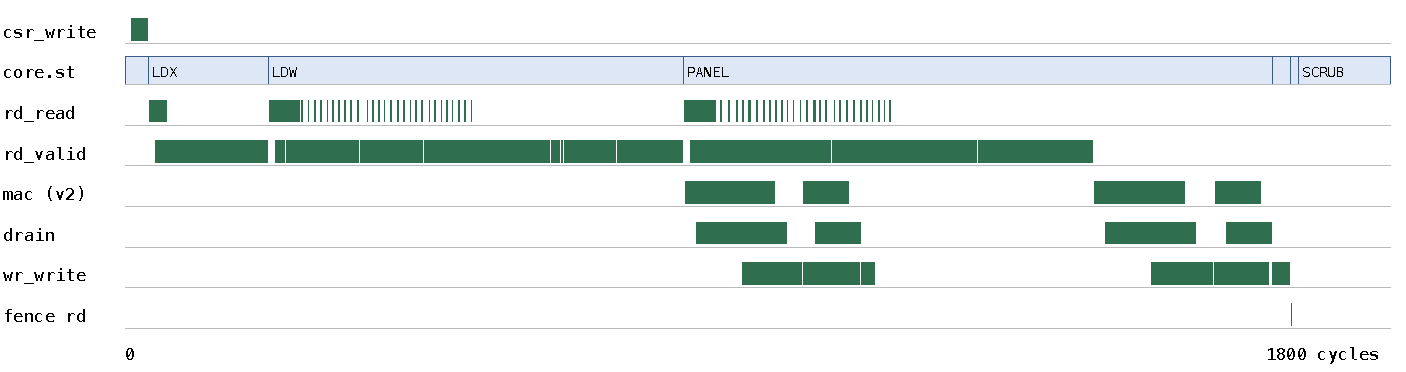
\includegraphics[width=\linewidth]{figs/fig3_wave.pdf}
\caption{Waveform (Icarus + GTKWave, \texttt{fpga/tb/lmm.gtkw}) untuk GEMM M=9, K=64, N=64, stall 20\%, latensi 8. Urutannya: START, LDX, LDW, lalu PANEL (prefetch panel 1 bertumpuk dengan MAC, drain, dan tulis Y), fence read, SCRUB.}
\end{figure}

{\scriptsize
\begin{tabularx}{\linewidth}{|r|R|R|r|R|R|R|R|}
\hline
\hd{L} & \hd{Siklus total [U]} & \hd{Siklus MAC [U]} & \hd{Utilisasi} & \hd{Baca + tulis DDR [U]} & \hd{ms/call @100 MHz} & \hd{BW rata-rata} & \hd{44 call: waktu / traffic} \\ \hline
109 & 1.586.114 & 1.548.288 & 97,6\% & 3,71 + 1,00 MB & 15,9 & 297 MB/s & 0,70 s / 207 MB \\ \hline
173 & 2.492.738 & 2.433.024 & 97,6\% & 7,34 + 1,59 MB & 24,9 & 359 MB/s & 1,10 s / 393 MB \\ \hline
301 & 4.297.754 & 4.202.496 & 97,8\% & 11,08 + 2,77 MB & 43,0 & 322 MB/s & 1,89 s / 610 MB \\ \hline
557 & 7.907.700 & 7.741.440 & 97,9\% & 18,55 + 5,13 MB & 79,1 & 300 MB/s & 3,48 s / 1.042 MB \\ \hline
\end{tabularx}

Siklus MAC sama persis dengan rumus $\lceil L/4\rceil\cdot(N/8)\cdot(K/4)$, dan byte baca/tulis sama dengan X + $\lceil L/128\rceil\cdot$W + Y. Waktu dalam ms adalah siklus terukur dikali clock asumsi; ini bukan waktu FPGA terukur.

\textbf{Sweep bandwidth DDR bersama} (token bucket R+W, arbitrasi round-robin seperti MPFE) [U]. Overhead terhadap compute murni untuk L=109 / 557:

\begin{tabular}{|r|r|r|}
\hline
\hd{Bandwidth efektif} & \hd{L=109} & \hd{L=557} \\ \hline
800 MB/s & 2,2\% & 2,0\% \\ \hline
500 MB/s & 3,3\% & 4,7\% \\ \hline
300 MB/s & 5,2\% & 13,5\% \\ \hline
200 MB/s & 54\% & 54\% \\ \hline
\end{tabular}

Pada 200 MB/s hasilnya 0,7\% dari batas teoretis \code{traffic/BW}, jadi perilakunya mengikuti \code{max(compute, transfer)}. Bila read diberi prioritas mutlak, overhead pada 800 MB/s naik ke 24\%. Konsekuensinya, bobot port MPFE harus diatur di board (temuan desain).}

\textbf{Uji board DE10-Nano (rencana):}
\begin{enumerate}
\item Platform Designer: HPS dengan F2S port0 RO-64 dan port1 RW-64, LW $\rightarrow$ CSR, \code{f2h\_irq0}.
\item Sintesis, fit, dan TimeQuest pada 100\,MHz.
\item \code{fpgaportrst} di U-Boot, lalu \code{laya\_mm.ko}.
\item Replay 72 fixture (bit-exact) dan test negatif di board.
\item Bandingkan dengan GEMM INT16 HPS-only (C+NEON) pada data yang sama.
\item SignalTap pada state, beat, dan stall.
\item Daya 5\,V lewat meter inline: idle, aktif, dan energi per call.
\end{enumerate}

{\scriptsize
\begin{tabularx}{\linewidth}{|p{0.3\linewidth}|L|}
\hline
\hd{Metrik keberhasilan} & \hd{Target} \\ \hline
Integer & 0 mismatch di simulasi dan board \\ \hline
Keputusan & 12/12 sama dengan baseline; max$|\Delta p|$ $\le$ 0,01 \\ \hline
Keamanan & 100\% test negatif ditolak tanpa transaksi bus \\ \hline
Throughput & $\ge$ 90\% dari 128 MAC $\times$ $f_\mathrm{clk}$ pada L=557 \\ \hline
Timing & slack positif di semua corner \\ \hline
Energi & J/inferensi kernel $<$ HPS-only (diukur, bukan diasumsikan) \\ \hline
\end{tabularx}

\textbf{Estimasi pembanding (belum diukur).} GEMM INT16 HPS-only dengan asumsi 0,5--3 GMAC/s [A] butuh 14--87\,s untuk 44 call pada L=557, sedangkan LMM-16 butuh 3,48\,s. Dengan daya board dari [1], energi diperkirakan $\approx$26\,J vs 54--323\,J, jadi keunggulan $\approx$2--12$\times$ [E] hanya di level kernel.}

% ---------------------------------------------------------------
\section{4. Referensi}
{\scriptsize
\begin{enumerate}[leftmargin=4.5mm]
\item R. Gadea-Giron\'es, J. L. Rocabado-Rocha, J. Fe, J. M. Monzo, ``A Heterogeneous Inference Framework for a Deep Neural Network,'' \emph{Electronics} 13(2):348, 2024, doi:10.3390/electronics13020348 (DE10-Nano: Tabel 8--10 latensi, resource, daya).
\item R. G. Molanes, J. J. Rodr\'iguez-Andina, J. Fari\~na, ``Performance Characterization and Design Guidelines for Efficient Processor--FPGA Communication in Cyclone V FPSoCs,'' \emph{IEEE Trans. Ind. Electron.} 65(5):4368--4377, 2018, doi:10.1109/TIE.2017.2766581; data: github.com/UviDTE-FPSoC/CycloneVSoC-time-measurements.
\item Intel, \emph{Cyclone V Device Datasheet} CV-51002, 2019.11.27, Tabel 32 (performa DSP), Tabel 40 (clock HPS).
\item Intel, \emph{Cyclone V Device Overview} CV-51001/683694, 2018.05.07 (Tabel 10, 16, 17; bridge HPS--FPGA; SDRAM 400 MHz); Altera WP-01159 (variable-precision DSP); \emph{Introduction to Cyclone V HPS} cv\_54001, 2014.02.28 (F2S: AXI-3/Avalon, $\le$ 6 port, 32--256 bit; LW 0xFF20\_0000).
\item R. Novickis, M. Greit\=ans, ``FPGA Master based on chip communications architecture for Cyclone V SoC running Linux,'' CoDIT 2018, pp. 403--408, doi:10.1109/CODIT.2018.8394842.
\item Terasic/Intel, \emph{DE10-Nano Get Started Guide} (A9 800 MHz, 1 GB DDR3 32-bit); Linux \texttt{drivers/fpga/altera-fpga2sdram.c} (FPGAPORTRST).
\item Y. Bondarenko, M. Nagel, T. Blankevoort, ``Understanding and Overcoming the Challenges of Efficient Transformer Quantization,'' EMNLP 2021, arXiv:2109.12948.
\item T. Dettmers et al., ``LLM.int8(): 8-bit Matrix Multiplication for Transformers at Scale,'' NeurIPS 2022, arXiv:2208.07339.
\item Laya: github.com/NandhaKishorM/laya; model convaiinnovations/laya (multilingual). Hasil repo ini: \texttt{profiling\_v2/}, \texttt{verification\_v1\_results/}, \texttt{fpga/results/}.
\end{enumerate}}

% ---------------------------------------------------------------
\section{5. Lampiran}
{\scriptsize
\noindent
\begin{minipage}[t]{0.485\linewidth}
\subsection{Tim \& Pembagian Peran}
\begin{tabularx}{\linewidth}{|p{0.2\linewidth}|p{0.18\linewidth}|L|}
\hline
\hd{Nama} & \hd{Keahlian} & \hd{Peran} \\ \hline
[Ketua] & [\dots] & RTL \& integrasi Platform Designer \\ \hline
[Anggota 1] & [\dots] & driver Linux, HPS baseline \\ \hline
[Anggota 2] & [\dots] & verifikasi, daya, laporan \\ \hline
\end{tabularx}

\subsection{Luaran \& Demo}
\begin{itemize}
\item \textbf{Repository:} \texttt{fpga/rtl} (585 baris), \texttt{fpga/tb}, \texttt{fpga/sw} (reference, gate, harness), dan hasil JSON. \texttt{.sof/.rbf} dibuat saat bootcamp.
\item \textbf{Demo live:} replay fixture Laya di board (bit-exact), test negatif keamanan, serta pembacaan PERF dan daya.
\item \textbf{Video 3--5 menit:} alur request dan waveform.
\end{itemize}
\end{minipage}\hfill
\begin{minipage}[t]{0.485\linewidth}
\subsection{Rencana Bootcamp (3 Hari)}
\begin{tabularx}{\linewidth}{|c|L|p{0.3\linewidth}|}
\hline
\hd{Hari} & \hd{Fokus} & \hd{Target} \\ \hline
1 & Quartus fit/timing, HPS + F2S, \texttt{fpgaportrst}, driver & GEMM kecil bit-exact di board \\ \hline
2 & Replay 72 fixture, HPS-only C/NEON, SignalTap & tabel siklus/latensi/BW terukur \\ \hline
3 & Daya \& energi, test negatif di board, demo & laporan teknis, video \\ \hline
\end{tabularx}

\subsection{Risiko \& mitigasi}
\begin{itemize}
\item \textbf{Bring-up F2S/\texttt{fpgaportrst}.} Mitigasi: jalur cadangan F2H, dengan kontrak RTL tetap.
\item \textbf{Fmax $<$ 100 MHz.} Mitigasi: tambah stage pipeline dot4.
\item \textbf{Arbitrasi DDR.} Mitigasi: atur bobot MPFE, atau perbesar obuf.
\item \textbf{Runtime ARMv7 untuk e2e.} Mitigasi: demo tingkat kernel.
\item \textbf{Quartus tidak ada di macOS.} Mitigasi: host x86.
\end{itemize}
\end{minipage}}

\end{document}
